\section{HomeActivity}
The \activity{HomeActivity} implements the app management described in \autoref{sec:app_manangement}. 
As seen in \autoref{fig:appmanagement_design} in \nameref{sec:app_management}, there are three branches of interaction. 
One of these is the \emph{Launch app} functionality.
A prerequisite of launching an app, is that the app is available to the user. 
To find out which apps to load, two lists of apps are retrieved. 
The first is the apps attached to the user in the Oasis database, and the second is the apps installed on the device.
The apps to be loaded are computed by taking the intersection of these two lists.

This ensures users are not allowed access to apps on the device they are restricted from.

The launcher does not ensure that apps are installed. 
A consequence hereof is that even if a user has permission to access an app, it will not be accessible if not installed.

\subsection{Drawer}
The drawer is implemented as described in \autoref{sec:drawer}.
The implemented design can be seen in \autoref{fig:home-activity_closed} and \autoref{fig:home-activity}.

\begin{figure}[h!]
	\centering
	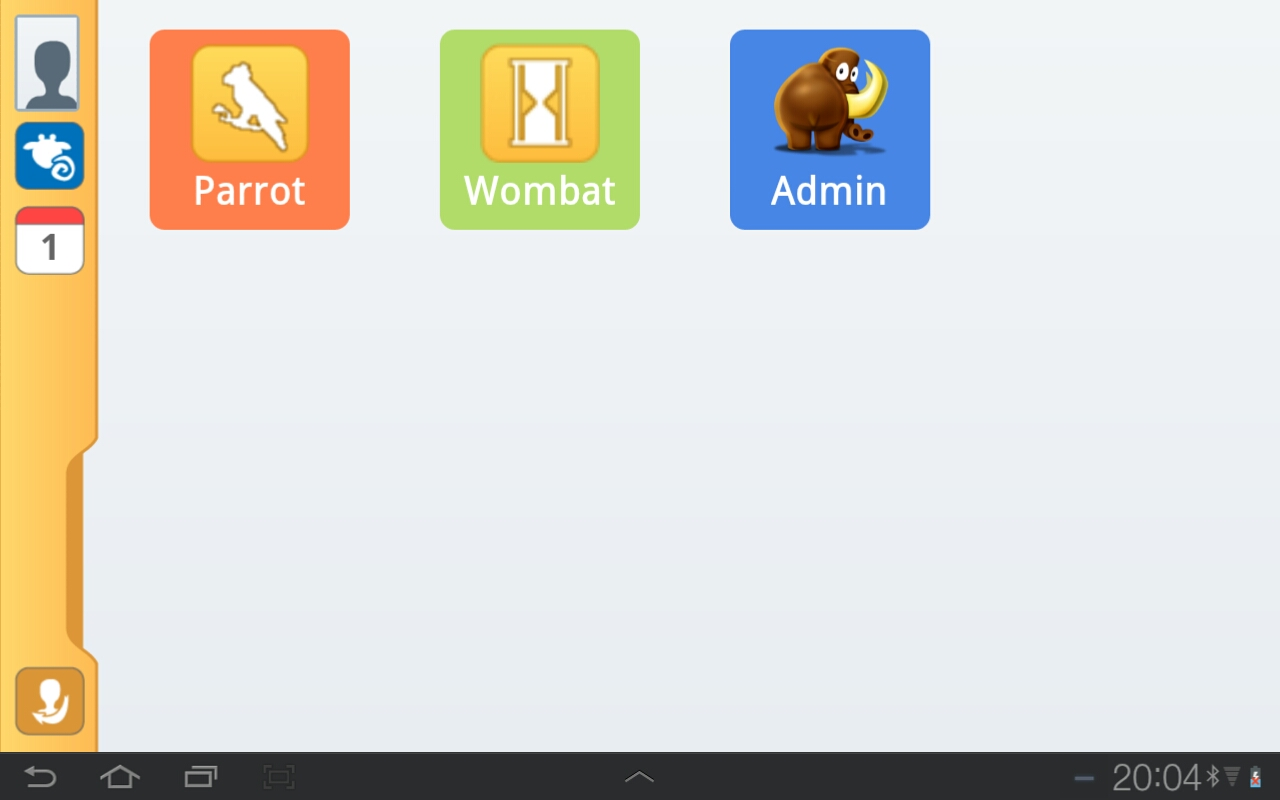
\includegraphics[width=0.7\textwidth]{gfx/implementation-home-drawerclosed}
	\caption{Shows the launcher with the drawer closed}
	\label{fig:home-activity_closed}
\end{figure}

\begin{figure}[h!]
	\centering
	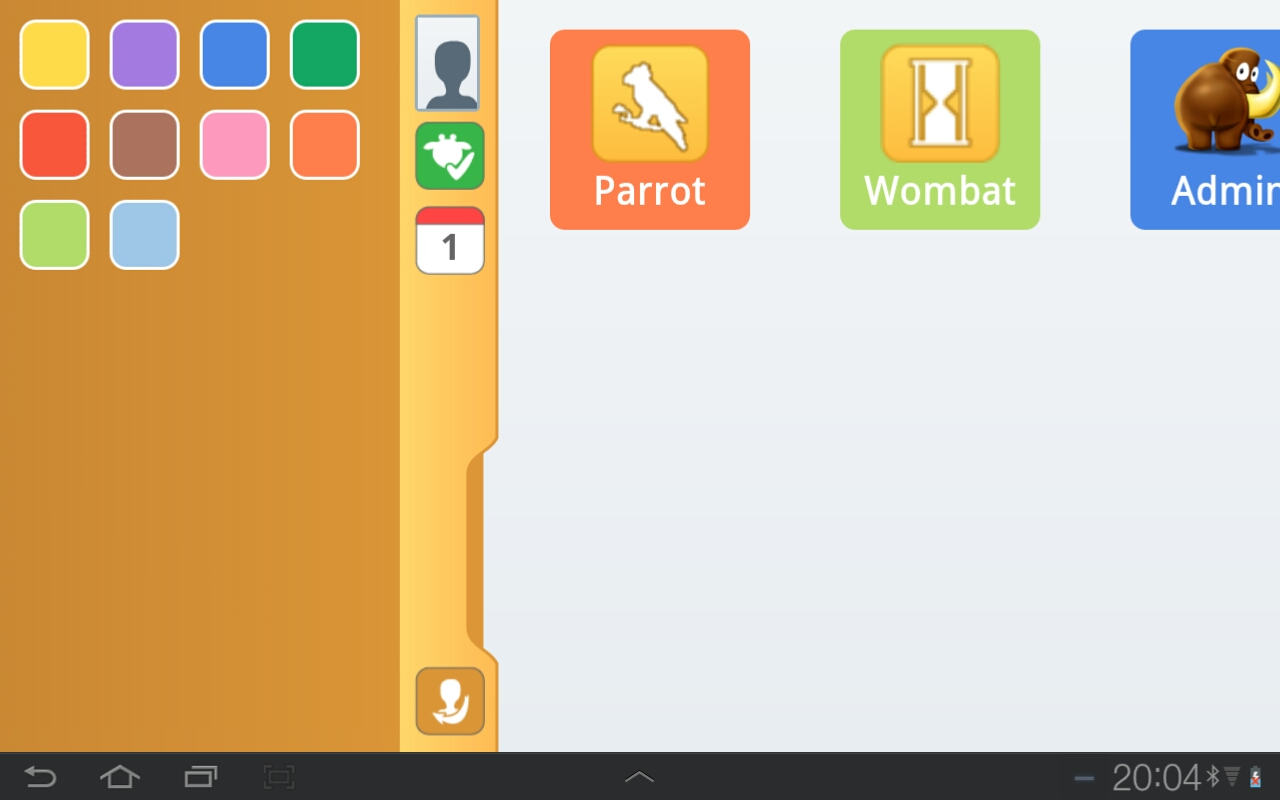
\includegraphics[width=0.7\textwidth]{gfx/implementation-home-draweropen}
	\caption{Shows the launcher with the drawer opened}
	\label{fig:home-activity}
\end{figure}

\subsection{Color picker}
\label{home:colorpicker}	
We believe that usability of the color picker can be heightened by further development on the class shown in \autoref{lst:draganddrop}.
The drag cases can be further developed to improve usability, as they can e.g. be used to indicate that the apps are able to recieve the dragged view, e.g. a color.

\begin{lstlisting}[style=sourceCode, language=JAVA, caption=The GAppdragger class, label=lst:draganddrop] 
public class GAppDragger implements OnDragListener {
	@Override
	public boolean onDrag(View view, DragEvent drawEvent) {
		switch(drawEvent.getAction()){
		case DragEvent.ACTION_DRAG_STARTED:
			break;
		case DragEvent.ACTION_DRAG_ENTERED:
			/*
			 * Future todo: implement highlighting
			 */
			break;
		case DragEvent.ACTION_DRAG_EXITED:
			/*
			 * Future todo: implement dehighlighting
			 */
			break;
		case DragEvent.ACTION_DROP:
			long id = Long.parseLong((String)view.getTag());
			int color = (int) Integer.parseInt(drawEvent.getClipData().getItemAt(0).getText().toString());
			
			AppAdapter.saveAppBackground(view.getContext(), view, color, id);
			break;
		case DragEvent.ACTION_DRAG_ENDED:
			/*
			 * Future todo: implement dehighlighting
			 */
			break;
		}
		return true;
	}
}
\end{lstlisting}

\subsection{Widgets}
The widgets are implemented in the \guicomponents[] library, and built as isolated classes such that they can be utilized in differents contexts. 
As widgets might need updates, we have implemented a periodic update mechanism, that updates \giraf[] widgets in a uniform manner.
This manner refers to all widgets being updated by a central updater, instead of running multiple clocks to update widgets seperately.
This behavior is enforced by having all widgets in \giraf[] implement the IGWidget-interface, and any widget to be updated should be added to the central updater.